
\title{Recap Database (02LSZOA)}
\author{Jacopo Nasi\\
        Computer Engenieer\\
        Politecnico di Torino}
\date{II Periodo - 2016/2017\\\bigskip\bigskip\today}

\documentclass[12pt]{article}
\usepackage[utf8]{inputenc}
\usepackage{geometry}
\usepackage{mathtools}
\usepackage{graphicx}
\usepackage{float}
\usepackage{amssymb}
\usepackage{ifsym}
% Misure Documento
\geometry{ a4paper, total={170mm,257mm},left=35mm, right=35mm, top=35mm, bottom=35mm }

\begin{document}

\begin{figure}
  \centering
  
\includegraphics[width=10cm]{images/polito.pdf}
\end{figure}

\maketitle
\newpage
\tableofcontents

\newpage
{\noindent \Large \textbf{License}\bigskip}

This work is licensed under a Creative Commons Attribution-NonCommercial-ShareAlike 3.0 Unported License.\\
You are free:
\begin{itemize}
  \item \textbf{to Share}: to copy, distribute and transmit the work
  \item \textbf{to Remix}: to adapt the work
\end{itemize}
Under the following conditions:
\begin{itemize}
  \item \textbf{Attribution}: you must attribute the work in the manner specified by the author or licensor (but not in any way that suggests that they endorse you or your use of the work)
  \item \textbf{Noncommercial}: you may not use this work for commercial purposes.
  \item \textbf{Share Alike}: if you alter, transform, or build upon this work, you may distribute the resulting work only under the same or similar license to this one.
\end{itemize}

\noindent More information on the Creative Commons website (http://creativecommons.org).

\begin{figure}[h!]
  \centering
  
\includegraphics[width=3cm]{images/license.png}
\end{figure}

{\noindent \Large \textbf{Acknowledgments}\bigskip}

Questo breve riepilogo non ha alcuno scopo se non quello di agevolare lo studio di me stesso, se vi fosse di aiuto siete liberi di usarlo.\\
Le fonti su cui mi sono basato sono quelle relative al corso offerto (\textbf{Database (02LSZOA)}) dal Politecnico di Torino durante l'anno accademico 2016/2017.\\
Non mi assumo nessuna responsabilità in merito ad errori o qualsiasi altra cosa. Fatene buon uso!
\newpage

\section{Introduction}\label{intro}
Everydays in our life we need to use data and the database are the structure to it in a computer-way.
\subsection{Introduction to database}

\paragraph{Information management}
Informations are recorded and exchanged in different forms.\\
\textit{The data are rough symbols which have to be interpreted and correlated to provide information.}\\
The data are far more stable over time than the process that manage them, the bank structure hasn't change for decades instead the procedures that manage the data are changeing often.

\paragraph{Database}
There are two definitions of \textit{database}:
\begin{itemize}
  \item \textbf{General}: collection of data that represents information interesting for a computer system.
  \item \textbf{Technical}: collection of data managed by a DBMS.
\end{itemize}

The \textbf{DBMS} (\textit{DataBase Management System}) is a software system able to manage collections of data (large, shared and persistent) ensuring the reliability and privacy. The main part of data is stored in the secondary memory.\\
The DB is an integrated resource, shared by several company sectors and the objective are:
\begin{itemize}
  \item Reduction of data redundancy.
  \item reduction of data inconsistency.
  \item competing acces control mechanism.
\end{itemize}
Other importart characteristics are:
\begin{itemize}
  \item \textbf{Data Persistance}: the lifetime is not limited to execution of programmes that use them.
  \item \textbf{Reliability}: backup and recovery functionality.
  \item \textbf{Privacy}
  \item \textbf{Efficency}: Capacity to carry out operations using a set of acceptable rescources for user.
  \item \textbf{Efficacy}: Capacity to render user activities productive.
\end{itemize}

The DBMS is an "extension" of the File System with more integrated services.

\paragraph{Data model}
The data model is a set of concepts utilized for organizing and describing a structure of data in a way understandable by a computer. This model build the relations to organize the data into sets of homogenous records (table).

\begin{center}
\begin{tabular}{ |c|c|c| }
 \hline
 \textbf{Code} & \textbf{Name} & \textbf{TeacherID} \\
 \hline
 \hline
 M2170 & Information Systems & D101\\
 \hline
 M4880 & Computer Networks & D102\\
 \hline
 F0410 & Databases & D321\\
 \hline
\end{tabular}
\end{center}

\begin{center}
\begin{tabular}{ |c|c|c|c| }
 \hline
 \textbf{ID} & \textbf{Name} & \textbf{Deparment} & \textbf{Phone\#} \\
 \hline
 \hline
 D101 & Green & Computer Engeneering & 123456\\
 \hline
 D102 & White & Telecomunications & 978965\\
 \hline
 D321 & Black & Computer Engeneering & 456545\\
 \hline
\end{tabular}
\end{center}

Before the relational model other model, near to the physical, were used like hierarchical or network. Now we use Object o XML.\\
The \textit{schema} is what describe the structure of the data, is not changing over time and is represented by the heading of each table. THe schema of the previous table are:
\begin{center}
\begin{tabular}{ |c|c|c| }
 \hline
 \textbf{Code} & \textbf{Name} & \textbf{TeacherID} \\
 \hline
\end{tabular}
\end{center}

\begin{center}
\begin{tabular}{ |c|c|c|c| }
 \hline
 \textbf{ID} & \textbf{Name} & \textbf{Deparment} & \textbf{Phone\#} \\
 \hline
\end{tabular}
\end{center}

The \textit{instance} is the content of each table and is rapidly variable and represented by the row in the table.\\
The are tow models:
\begin{itemize}
  \item \textbf{Conceptual}: Can rappresente data independently from the logical and it describe real world concepts (used in the desing phase).
  \item \textbf{Logical}: Describe the data structure in the DBMS and is used by programmes to accessing the data and it's indipendent from the physical structures.
\end{itemize}

\paragraph{Data independence}
Is an important characteristics, it guarantees that users and programeers which utilize a database can ignore the designing details used n the constructions of the database.\\
The \textbf{physical independence} enables interaction with the DBMS independently from the physical structure of the data and for the external level too and allows to change the way the data is physically stored without affecting the software that utilizing it.\\
The \textbf{logical independence} enables interaction with the external level independently from the logical, allow the modifications on the logial level maintaining the external structures unaltered and is possibile to add new views without changing the logial schema.

\paragraph{Data access}
The language used for the data access is user-friendly, interactive (SQL) and the commands are able to interact with other languages with, the programmer, are able to develop specific functionalities.\\
There are 2 types of languages:
\begin{itemize}
  \item \textbf{DDL} (\textit{Data Definition Languages}): Used to define the logical, external and physical schemas and access authorizations.
  \item \textbf{DML} (\textit{Data Manipulation Languages}): Used for querying and updating database instances.
\end{itemize}

\noindent There are multiple roles in the system organizations:
\begin{itemize}
  \item \textbf{Administrator}: Control and management of the database (performance, reliability, auth, ecc...).
  \item \textbf{Programmer}: Define and realize the structure of the db.
  \item \textbf{User}: Use software with predefined activities (end) or formulate queries not predefined (casual).
\end{itemize}

\paragraph{DBMS pro \& cons}
The main advantages are:
\begin{itemize}
  \item Data as a common resource.
  \item Unified and precise data model.
  \item Centralizable.
  \item Data independence.
\end{itemize}
the disadvantages are:
\begin{itemize}
  \item Expensive with product purchase.
  \item Provide a set of service in an integrated form and is not possibile to separated the unused ones.
\end{itemize}

\section{Relational data model and algebra}
\subsection{Relational Data Model}
\paragraph{Introduction}
It was proposed around 1970 to support higer abstract levels compared to the previous model. Is now the main model exploited in commercial DBMSs.
\paragraph{Definition}
The are some important word:
\begin{itemize}
  \item \textbf{Attribute}: Column of a table.
  \item \textbf{Domain}: Value set that can be assumed by an attribute.
  \item \textbf{Tuple} (or record): A row in a table.
  \item \textbf{Cardinality}: Number of tuples in a relation.
  \item \textbf{Degree}: Numbers of attributes in a relation.
\end{itemize}
We need to remember that attributes and tuples are not ordered and are distinct.

\paragraph{Reference between relations}
The relational model is value-based and the references between data in different relations are represented by means of values of the domains. This allows the independence od physical structures, only relevant information are stored, it's easy to be transferred and the link is not oriented.

\paragraph{Null values}
Some information could be not available for ani tuples in the relation, for a student table, for example, the DegreeYear it could be not yet defined, or others like this...\\
Is a good practise to used a special vaue belonging to the domain to represente the lack of information. The \textit{null value} is not a good choice because is not a value of the domain and in means the absence of both value and domain.

\paragraph{Integrity Constraints}
Are property that must be satisfied by all database instances, they can be \textbf{Intra-relation} constraints defined on the attributes of a single relation (ex: unique constraints, domain constraints, tuple constraints) or \textbf{Inter-realation} constraints defined in many relations at the same time (ex: referential constraint).

\paragraph{Primary Key}
Is an attribute set that uniquely identifies tuples in a relation in the students case for example there is no pair of students with the same value for StudentID. Are unique and minimal, there exists no other key that are contained in a subset of the key. The primary key can be made by multiple NON UNIQUE keys. It can't assume the \textit{null value}.

\paragraph{Tuples, domain and referential constraint}
These are condition over data, a domain constraint express the conditions on the value assumed by an attribute of a tuple, the tuple constraint express conditions on the values of each tuple indipendently of other tuples. The referential constraint are between more table, an attribute (external) of the A table refers to a key (internal) in the B table that must be exist. The realational constraint are imposed in order to guarantee that the values refer to actual values in the referenced relation.

\subsection{Relational Algebra}
\paragraph{Introduction}
This algebra extend algebra of sets for the relational model and defines a set of operators that operate on relations and whole result is a relation.\\
There are 2 kind of division for the operator:
\begin{itemize}
  \item \textbf{Unary Operator}
  \begin{itemize}
    \item Selection ($\sigma$)
    \item Projection ($\pi$)
  \end{itemize}
  \item \textbf{Binary Operator}
  \begin{itemize}
    \item Cartesian Product (x)
    \item Join ($\bowtie$)
    \item Union ($\cup$)
    \item Intersection ($\cap$)
    \item Difference ($-$)
    \item Division ($/$)
  \end{itemize}
\end{itemize}
or in this mode:
\begin{itemize}
  \item \textbf{Set Operator}
  \begin{itemize}
    \item Union ($\cup$)
    \item Intersection ($\cap$)
    \item Difference ($-$)
    \item Cartesian Product (x)
  \end{itemize}
  \item \textbf{Binary Operator}
  \begin{itemize}
    \item Join ($\bowtie$)
    \item Selection ($\sigma$)
    \item Projection ($\pi$)
    \item Division ($/$)
  \end{itemize}
\end{itemize}

\paragraph{Selection} extract a ``horizontal'' subset from the relation. For the query: \textit{"Find the courses held in the second semester"} the result will be like the figure \ref{fig:select}.\\
The selection generate a relation R:
\begin{itemize}
  \item With the same schema as A.
  \item Containing all the tuples of relation A because of which predicate \textit{p} is true.
\end{itemize}
The literal relation is $R=\sigma_{p}A$ in this case A is the table Courses and the predicate \textit{p} is semester=2.
\begin{figure}[H]
  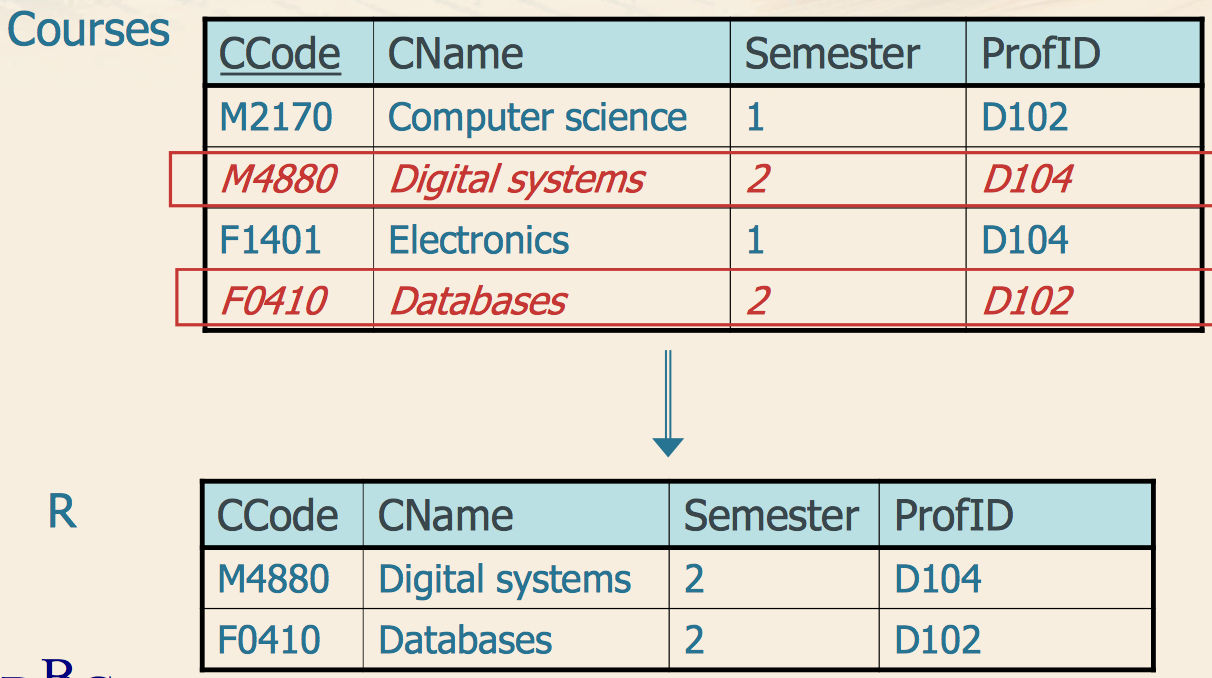
\includegraphics[width=\textwidth]{images/select.png}
  \caption{Selection}
  \label{fig:select}
\end{figure}

\paragraph{Projection} extracts a ``vertical'' subset of attributes from the relation. For the query: \textit{"Find the names of professors"} the result will be like figure \ref{fig:proj}.\\
The projection generate a relation R:
\begin{itemize}
  \item Whose schema is the list of attributes L.
  \item Containing all the tuples present in A.
\end{itemize}
The literal relation is $R=\pi_{L}A$ in this case A is the table Professors and the predicate is \textit{L} is PName. Is also possible to use \textit{Selection} and \textit{Projection} together.
\begin{figure}[H]
  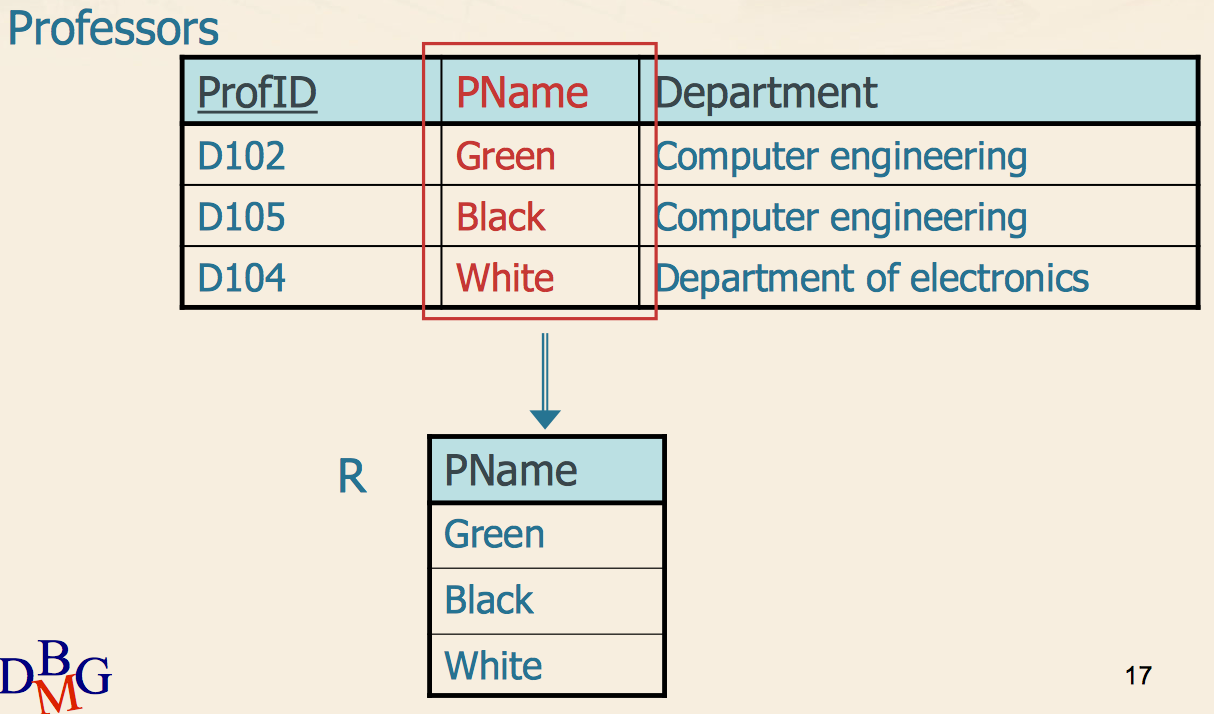
\includegraphics[width=\textwidth]{images/proj.png}
  \caption{Projection}
  \label{fig:proj}
\end{figure}

\paragraph{Cartesian Product} it generates all the pairs formed by all tuple of A and all tuple of B. The result for the query: \textit{"Find the cartesian product of courses and professor"} will generated a big relation with, for each tuple of A all the tuple of B. A relation with 3 tuples in A and 4 tuples in B, will give you a table of 12 tuples. The literal expression is $R=AxB$ and is commutative and associative.

\paragraph{Join} generate a relation with all pairs formed by a tuple of A and a tuple of B that are \textit{semantically linked}. The query: \textit{"Find information about courses and the professor that hold them"} will give you back a relation like figure \ref{fig:join}.\\
The join can be expressed like a mix of \textit{cartesian product, selection and projection}.\\
There are 3 different types of join:
\begin{itemize}
  \item \textbf{Natural}: $R=A\bowtie B$ (contains all the pairs with the same value of a given attribues)
  \begin{itemize}
    \item The attributes which are present in A's schema and not in B's.
    \item The attributes which are present in B's schema and not in A's.
    \item A single copy of common attributes.
  \end{itemize}
  \item \textbf{Theta}: $R=A\bowtie_{p} B$ (contains all the pairs with the same value of a given attribues that meet a predicate \textit{p})
  \begin{itemize}
    \item Whose schme ais the unione of the schemes of A and B.
    \item Containing all the pairs made up of a tuple of A and a tuple of B for which predicate ($X \theta Y$) is true.
  \end{itemize}
  \item \textbf{Equi}: $R=A\bowtie_{p} B$ (special case with $\theta$ is (=))
  \item \textbf{Semi}: $R=A\ltimes_{p} B$ (similar to theta but only with the attributes of A)
\end{itemize}
\begin{figure}[H]
  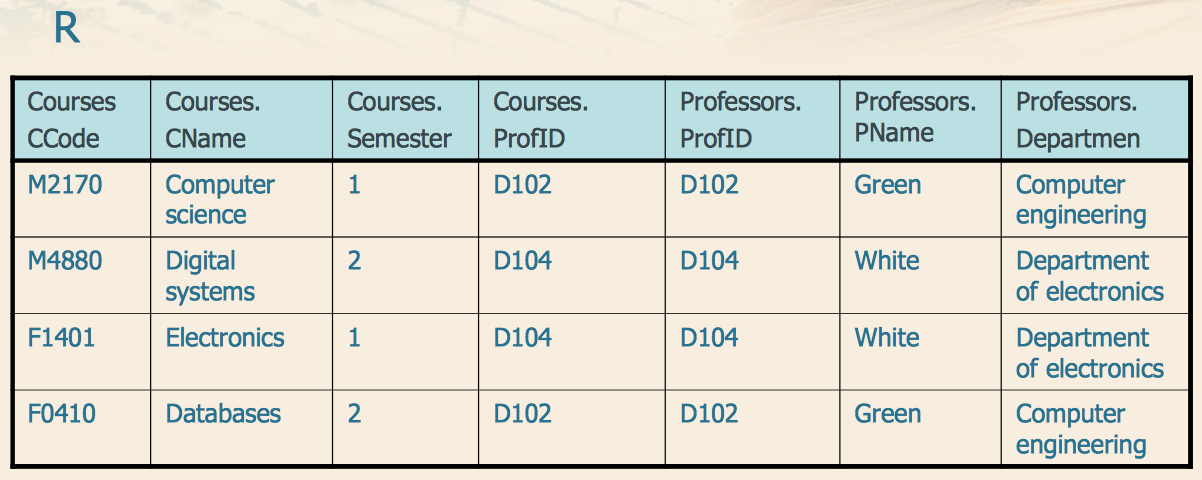
\includegraphics[width=\textwidth]{images/join.png}
  \caption{Join}
  \label{fig:join}
\end{figure}

\paragraph{Outer-join} is a version of join where you can conserve the information relative to tuples that are not semantically linked by the join predicate, the tuples will be completed with \textit{null value}. There are 3 types of outer-join:
\begin{itemize}
  \item \textbf{Left}: $R=A {\tiny \textifsym{d|><|}}_{p} B$ Are conserved the tuples of the left table, with null value for the attributes of the right part.
  \item \textbf{Right}: $R=A {\tiny \textifsym{|><|d}}_{p} B$ Are conserved the tuples of the right table, with null value for the attributes of the left part.
  \item \textbf{Full}: $R=A {\tiny \textifsym{d|><|d}}_{p} B$ Are conserved the tuples of both table.
\end{itemize}

\paragraph{Union} selects all the tuples present in at least one of the two (A and B) relations. If there are duplicated tuple this command will provide only one of this. The main characteristics are:
\begin{itemize}
  \item R has the same schema of A and B. (This means that both A and B must have the same schema)
  \item Containing all the tuples belonging to A and all the tuples belonging to B.
\end{itemize}
THe literal expression is $R=A \cup B$. For example the result of the query: \textit{"Find infomration relative to the profesors of degree or master courses"} will show to you the result of the figure \ref{fig:union}
\begin{figure}[H]
  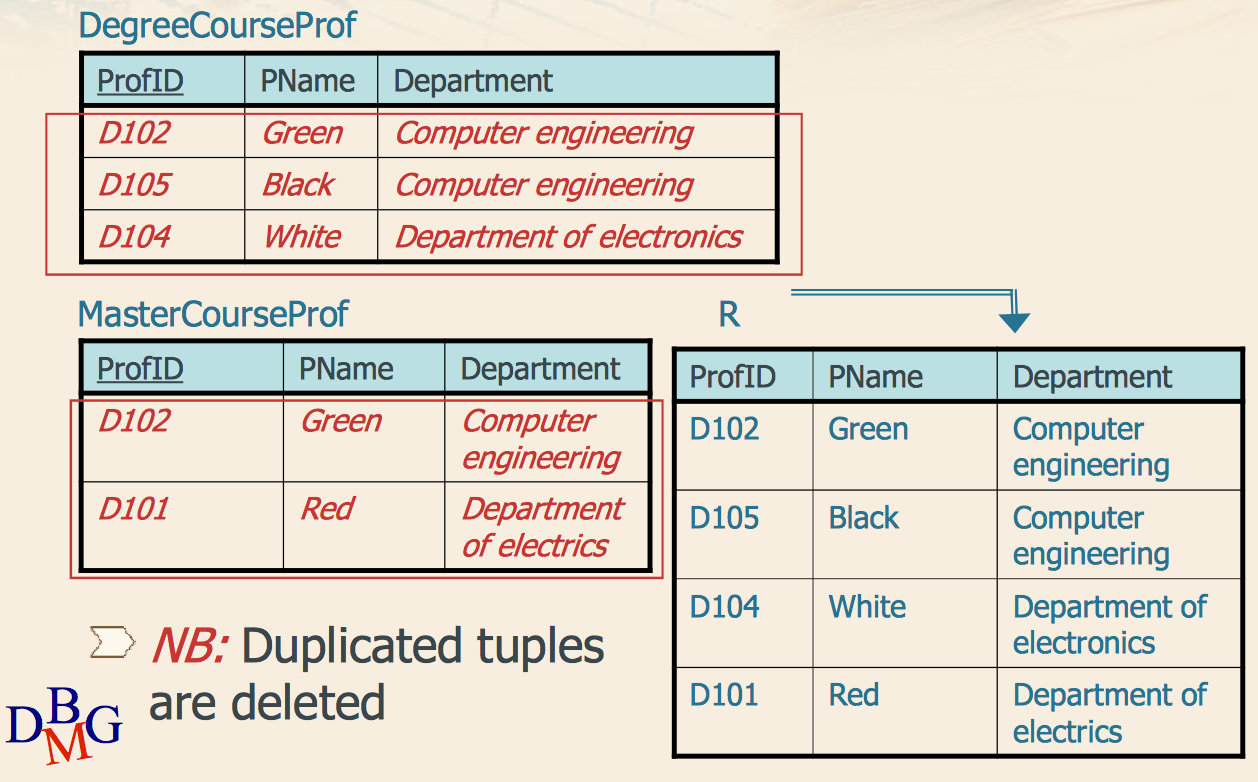
\includegraphics[width=\textwidth]{images/union.png}
  \caption{Union}
  \label{fig:union}
\end{figure}

\paragraph{Intersection} select only the tuples that are present on both table A and B. The main characteristics are:
\begin{itemize}
  \item R has the same schema of A and B. (This means that both A and B must have the same schema)
  \item Containing all the tuples belonging to both A and B.
\end{itemize}
THe literal expression is $R=A \cap B$.

\paragraph{Difference} this operator will extract only the tuples that are in the A but that are not in the B. A possibile query is: \textit{"Find the professors teaching degree courses but not master's"}. It has the same specs of the intersection or union, but is not commutative and associative.\\
Like the previous operator if the schemas are different you need to perform a projection before using it.

\paragraph{Anti-join} selects all tuples of A that are \textit{not semantically linked} to tuples of B. The information of the second table will not appear in the result. R will have the same schema of A and containing all the tuples of A for which there is no tuple of B for which the predicate \textit{p} is true.

\paragraph{Division} the division select all tuples of A that have a corrisponding value in B, is necessary that the A tuples have ALL the corresponding value of B.\\
If our query is: \textit{"Find all the student that have passed the exams of ALL courses of the first year"} the result will be like figures \ref{fig:div1} and \ref{fig:div2}.
\begin{figure}[H]
  \centering
  \begin{minipage}{.45\textwidth}
    \centering
    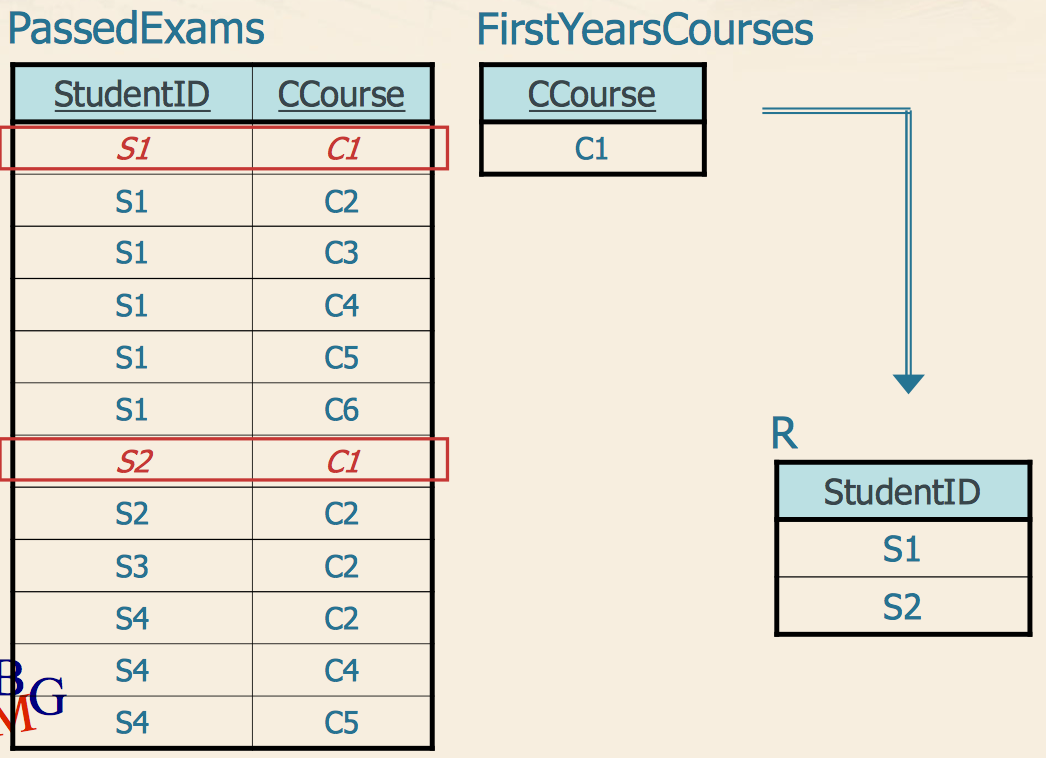
\includegraphics[width=\textwidth]{images/div1.png}
    \caption{Division 1st example}
    \label{fig:div1}
  \end{minipage}\hfill
  \begin{minipage}{.45\textwidth}
    \centering
    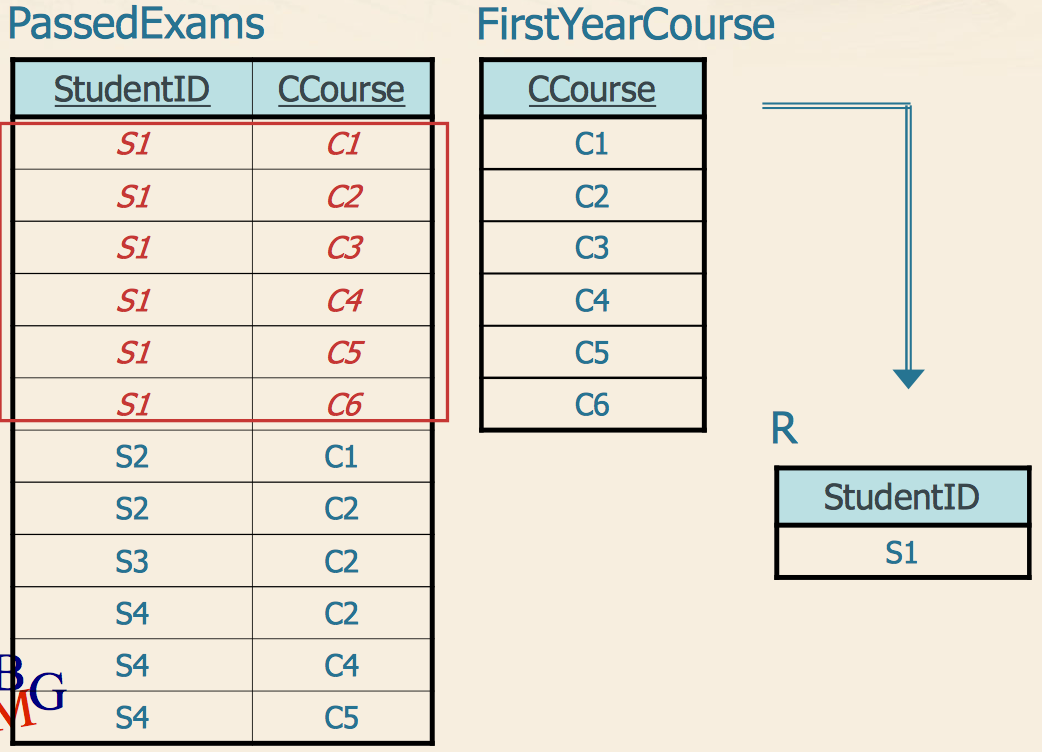
\includegraphics[width=\textwidth]{images/div2.png}
    \caption{Division 2nd example}
    \label{fig:div2}
  \end{minipage}\hfill
\end{figure}

% Giovedì 9 Marzo 15:22

% \section{SQL Language}
% \subsection{Introduction}

\bibliographystyle{abbrv}
\bibliography{simple}

\end{document}
